\begin{figure}[H]
\centering
\includegraphics[width=0.48\textwidth]{\FCNCFigures/tthML/originFit/reg2l1tau1bnj_vetobtagwp70_highmet/tau_pt_0.pdf}
\includegraphics[width=0.48\textwidth]{\FCNCFigures/tthML/originFit/reg2l1tau2bnj_vetobtagwp70_highmet/tau_pt_0.pdf}

\includegraphics[page=6,width=0.48\textwidth]{\FCNCFigures/tthML/originFit/reg1l1tau2b2j_os_vetobtagwp70_highmet/tau_pt_0.pdf}
\includegraphics[page=6,width=0.48\textwidth]{\FCNCFigures/tthML/originFit/reg1l1tau2b3j_os_vetobtagwp70_highmet/tau_pt_0.pdf}

\includegraphics[page=6,width=0.48\textwidth]{\FCNCFigures/tthML/originFit/reg1l1tau2b2j_ss_vetobtagwp70_highmet/tau_pt_0.pdf}
\includegraphics[page=6,width=0.48\textwidth]{\FCNCFigures/tthML/originFit/reg1l1tau2b3j_ss_vetobtagwp70_highmet/tau_pt_0.pdf}

\caption{经过Fake tau校准后的$t\bar{t}$控制区的$\tauhad$的$\pt$谱。如预期,本底估计的数据符合程度被大幅提升。}
\label{fig:wjet_pt_postfit_CR}
\end{figure}
